\newpage
\subsection{Visual Schema}
\visHeader

\begin{enumerate}

\item[$\blacktriangleright$] Open \texttt{LearningBox2Dictionary.eap} in EA, and add a new package to your model root with \texttt{Learning\-Box\-To\-Dictionary\-Integration} as its name. 
Create a diagram for the new package and select \texttt{TGGSchema} as diagram type (Fig.~\ref{fig:tgg_diagram_type}). 
The diagram type indicates that the new package is a TGG Project. 

\begin{figure}[htbp]
\begin{center}
  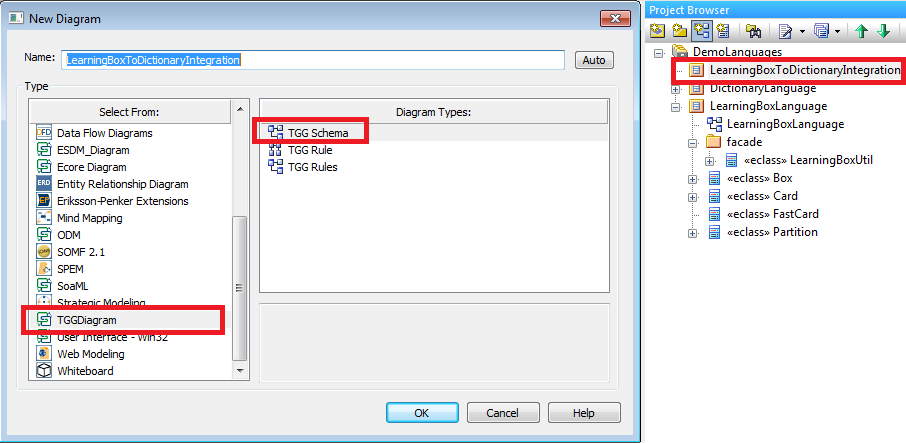
\includegraphics[width=\textwidth]{tgg1}
  \caption{Choose \texttt{TGGSchema} as your diagram type}  
  \label{fig:tgg_diagram_type}
\end{center}
\end{figure}

\item[$\blacktriangleright$] After choosing \texttt{TGGSchema} as diagram type, a new dialogue should pop up asking you for the source and target projects of your TGG project. 
Choose \texttt{Learning\-Box\-Language} as source and \texttt{Dictionary\-Language} as target project and affirm with \texttt{OK} (Fig.~\ref{fig:select_source_target}).

\begin{figure}[htbp]
\begin{center}
  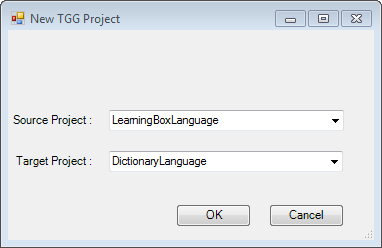
\includegraphics[width=0.55\textwidth]{tgg2.png}
  \caption{Select source and target projects for the TGG project}  
  \label{fig:select_source_target}
\end{center}
\end{figure}
\end{enumerate}

The structure of your TGG project should now resemble Fig.~\ref{fig:new_tgg_project}.
Please note that a subpackage \texttt{Rules} and an underlying diagram with the same name are also generated.

\begin{figure}[htbp]
\begin{center}
  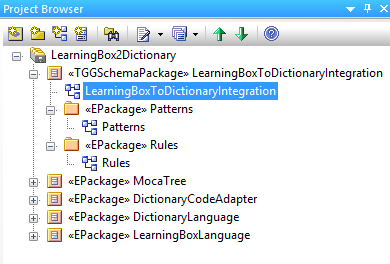
\includegraphics[width=0.5\textwidth]{tgg3.png}
  \caption{Initial structure of a new TGG project}  
  \label{fig:new_tgg_project}
\end{center}
\end{figure}

Now it's time to insert classes from our source and target projects into our TGG project and declare our first correspondence type between them.
The classes \texttt{Box} and \texttt{Dictionary}, both at the top of the composite hierarchy of their respecitve languages, are to be related to each other:
\begin{enumerate}
\item[$\blacktriangleright$] Drag \& drop the class \texttt{Box} in \texttt{Learning\-Box\-Language} from the project 
browser to the newly created TGG schema diagram \texttt{Learning\-Box\-To\-Dictionary\-Integration}.
Ensure that the class is pasted \texttt{as a simple link} into the diagram as depicted in Fig.~\ref{fig:drag_drop_box}. 
If the dialogue in Fig.~\ref{fig:drag_drop_box} doesn't show up and the element is pasted instead as an instance of the class, hold down \texttt{Ctrl} when dropping to invoke it.

\begin{figure}[htbp]
\begin{center}
  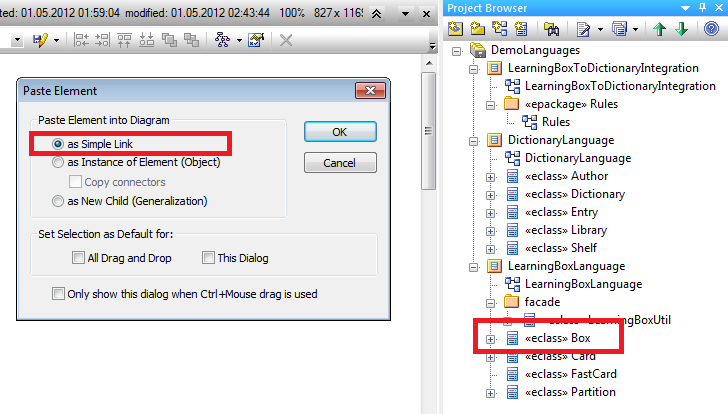
\includegraphics[width=0.83\textwidth]{tgg4.png}
  \caption{Drag \& Drop \texttt{Box} as a simple link into the TGG schema} 
  \label{fig:drag_drop_box}
\end{center}
\end{figure}

\item[$\blacktriangleright$] In the same way, drag \& drop the class \texttt{Dictionary} from \texttt{Dictionary\-Language} into the TGG schema. 
\end{enumerate}

With a class from both source and target projects, we can now create a correspondence type between them.
\begin{enumerate}
\item[$\blacktriangleright$] Quick link from \texttt{Box} to \texttt{Dictionary} and select \texttt{Create TGG Corres\-pon\-dence Type} as depicted in Fig.~\ref{fig:create_correspondence}.
\end{enumerate}

\begin{figure}[htbp]
\begin{center}
  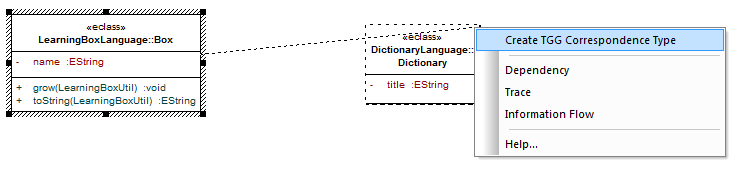
\includegraphics[width=\textwidth]{tgg5.png}
  \caption{Creating a TGG correspondence type} 
  \label{fig:create_correspondence}
\end{center}
\end{figure}

A hexagon-shaped correspondence type with the name \texttt{BoxToDiction\-ary} and references to the source and target elements should be generated.
You can rename the correspondence type as you wish but please leave the references as they are (multiplicity and naming conventions are satisfied automatically).

To complete our TGG schema, declare a further correspondence type between \texttt{Card} and \texttt{Entry}.
The complete TGG Schema is depicted in Fig.~\ref{fig:complete_tgg_schema}.

\begin{figure}[htbp]
\begin{center}
  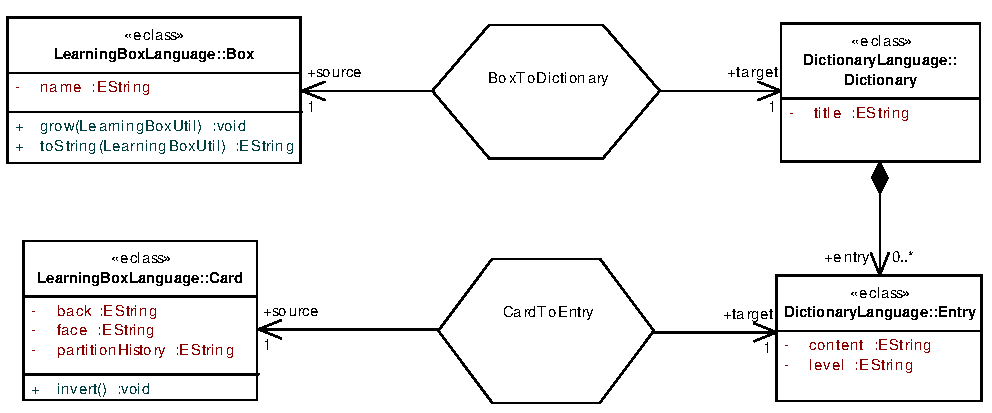
\includegraphics[width=\textwidth]{tgg7}
  \caption{Complete TGG schema for our example}
  \label{fig:complete_tgg_schema}
\end{center}
\end{figure}

